%%%%%%%% ICML 2018 EXAMPLE LATEX SUBMISSION FILE %%%%%%%%%%%%%%%%%

\documentclass{article}

% Recommended, but optional, packages for figures and better typesetting:
\usepackage{microtype}
\usepackage{graphicx}

\usepackage{subfig}
\usepackage{color}

% hyperref makes hyperlinks in the resulting PDF.
% If your build breaks (sometimes temporarily if a hyperlink spans a page)
% please comment out the following usepackage line and replace
% \usepackage{icml2018} with \usepackage[nohyperref]{icml2018} above.
\usepackage{hyperref}

% Attempt to make hyperref and algorithmic work together better:
\newcommand{\theHalgorithm}{\arabic{algorithm}}

% Use the following line for the initial blind version submitted for review:
\usepackage{sty_bst/icml}
\usepackage{booktabs} % for professional tables
\usepackage{amsmath}
\usepackage{amssymb}


% hyperref makes hyperlinks in the resulting PDF.
% If your build breaks (sometimes temporarily if a hyperlink spans a page)
% please comment out the following usepackage line and replace
% \usepackage{icml2018} with \usepackage[nohyperref]{icml2018} above.
\usepackage{hyperref}

\newcommand{\todo}[1]{\textcolor{red}{#1}}


% The \icmltitle you define below is probably too long as a header.
% Therefore, a short form for the running title is supplied here:
%\icmltitlerunning{Submission and Formatting Instructions for ICML 2018}

\begin{document}

\twocolumn[
\icmltitle{Neural Network Petridish}

% It is OKAY to include author information, even for blind
% submissions: the style file will automatically remove it for you
% unless you've provided the [accepted] option to the icml2018
% package.

% List of affiliations: The first argument should be a (short)
% identifier you will use later to specify author affiliations
% Academic affiliations should list Department, University, City, Region, Country
% Industry affiliations should list Company, City, Region, Country

% You can specify symbols, otherwise they are numbered in order.
% Ideally, you should not use this facility. Affiliations will be numbered
% in order of appearance and this is the preferred way.
\icmlsetsymbol{equal}{*}

\begin{icmlauthorlist}
\icmlauthor{Aeiau Zzzz}{equal,to}
\icmlauthor{Bauiu C.~Yyyy}{equal,to,goo}
\icmlauthor{Cieua Vvvvv}{goo}
\icmlauthor{Iaesut Saoeu}{ed}
\icmlauthor{Fiuea Rrrr}{to}
\icmlauthor{Tateu H.~Yasehe}{ed,to,goo}
\icmlauthor{Aaoeu Iasoh}{goo}
\icmlauthor{Buiui Eueu}{ed}
\icmlauthor{Aeuia Zzzz}{ed}
\icmlauthor{Bieea C.~Yyyy}{to,goo}
\icmlauthor{Teoau Xxxx}{ed}
\icmlauthor{Eee Pppp}{ed}
\end{icmlauthorlist}

\icmlaffiliation{to}{Department of Computation, University of Torontoland, Torontoland, Canada}
\icmlaffiliation{goo}{Googol ShallowMind, New London, Michigan, USA}
\icmlaffiliation{ed}{School of Computation, University of Edenborrow, Edenborrow, United Kingdom}

\icmlcorrespondingauthor{Cieua Vvvvv}{c.vvvvv@googol.com}
\icmlcorrespondingauthor{Eee Pppp}{ep@eden.co.uk}

% You may provide any keywords that you
% find helpful for describing your paper; these are used to populate
% the "keywords" metadata in the PDF but will not be shown in the document
\icmlkeywords{Machine Learning, ICML}

\vskip 0.3in
]

% this must go after the closing bracket ] following \twocolumn[ ...

% This command actually creates the footnote in the first column
% listing the affiliations and the copyright notice.
% The command takes one argument, which is text to display at the start of the footnote.
% The \icmlEqualContribution command is standard text for equal contribution.
% Remove it (just {}) if you do not need this facility.

%\printAffiliationsAndNotice{}  % leave blank if no need to mention equal contribution
\printAffiliationsAndNotice{\icmlEqualContribution} % otherwise use the standard text.

\begin{abstract}
Neural architecture search. Growing networks. Lifelong, continuous learning. 
Starting from existing networks.
\end{abstract}

\section{Introduction}

Deep neural networks have been the backbone of many advancement in practical machine learning applications. However, the architectures of neural networks has been until recently handcrafted by experts. 


We summarize our contribution as follows.
\begin{itemize}
\item We propose to incrementally add computational complexity to neural networks during architecture search, by initializing a diverse pool of candidate changes and selecting the most prominent ones at the same time through feature selection. 
\item Our search warm-starts with parameters of previous models, and we show this leads to more accurate performance estimation of architectures, which in turn results in faster searches.
\item By initializing and choosing from a diverse pool of candidate changes, we can grow network intelligently into cost-efficient models. We empirically demonstrate the advantage of feature selection over random selection of incremental changes. 
\item \todo{We show the incremental improvement can be applied to many existing models, including ...}  
\end{itemize}


\section{Background and References}
\begin{itemize}
    \item NAS. (RL. EA. Gradient based.) 
    \item (Micro. Macro.) 
    \item Multi objective NAS; Pareto Front Nas 
    \item Evaluation with few epochs vs many epochs
    \item Incremental training, AdaNet, Boosted ResNet, Net morphism
    
    \item Test~\cite{NAS, NASCell, Hsu2018MONASMN, Elsken2018NeuralAS, Real2018RegularizedEF, Liu2018DARTSDA, Kandasamy2018BNAS, Pham2018EfficientNA, Liu2017ProgressiveNA}
\end{itemize}



\section{Method}

\subsection{Overall Search Procedure}
\label{sec:search_procedure}

\begin{figure*}
    \centering
    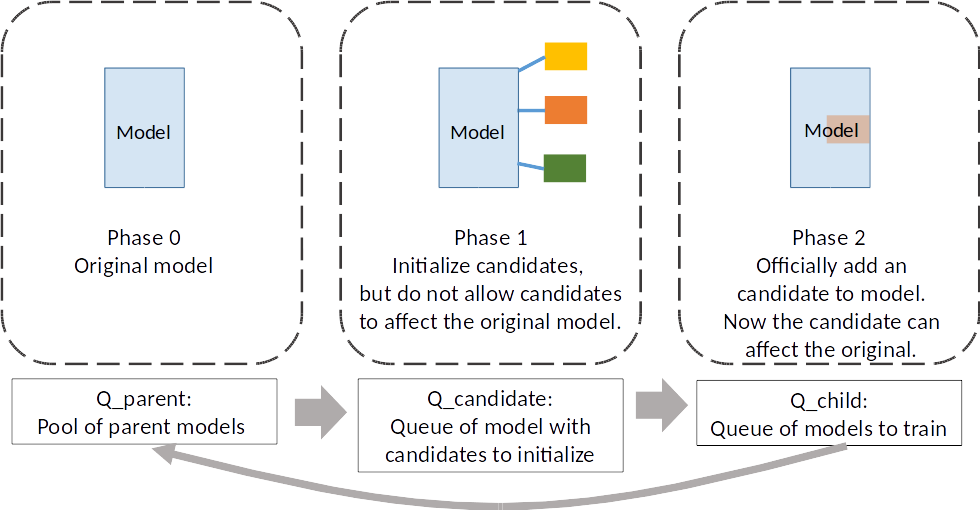
\includegraphics[width=0.8\textwidth]{img/three_queues.png}
    \caption{Caption}
    \label{fig:search_procedure}
\end{figure*}

Fig.~\ref{fig:search_procedure} describes search procedure as three steps: choosing parent models, initializing candidate layers, and training promising children models. The parent step selects from a pool of trained models, $Q_{p}$, a initial model $m$. The choice details are in Sec.~\ref{sec:parent_choice}. We modify $m$ into $m'$ by adding a number of candidate layers, and add $m'$ into a work queue, $Q_{c}$. The modifications are specified in Sec.~\ref{sec:hallu_choice}. The modified model $m'$ is initialized by workers for $Q_{c}$ through a few iterations of training, as detailed in Sec.~\ref{sec:hallu_init}. 
Based on statistics of the candidate layers, we only select some subsets of them to actually add to the parent model $m$ to form children models $m''_1$, $m''_2$, and so on. These children models are trained by workers of the children queue $Q_{c}$, starting from parameters of the parent and the candidate initialization. Children are added to $Q_p$, if they are cost-efficient. 

The above search procedure is similar to evolutionary algorithms (EA) based architecture search~\citep{Real2018RegularizedEF, Elsken2018EfficientMN}, since each of our model is modified from existing parent models. However, we have an additional initialization phase that train many potential children models jointly in one network model in order to select only few of them. Such approach of trying many and selecting few takes inspiration from model pruning~\citep{huang2017condensenet} and architecture search algorithms that prune model super-graphs~\citep{Pham2018EfficientNA, Liu2018DARTSDA}.




\subsection{Choice of Parent Models}
\label{sec:parent_choice}


Since the goal of our architecture search is to find the most cost-efficient models, we take a greedy approach to directly expand existing most cost-efficient models. The cost-efficiency is determined by the plot of model test-time computational cost versus their prediction error rates. The most cost efficient models lie on the Pareto-frontier of the plot, meaning there are no other models that are both cheaper and more accurate. Multiple previous works~\citep{Elsken2018EfficientMN, Hsu2018MONASMN} have studied expanding models on the frontier. 

Near the start of the architecture search, we may not have many points on the Pareto frontier. In fact, in our experiments, we start with one single initial model. This eases the design of the initial search condition, but poses a challenge for the algorithm to discover and expand the frontier. 




Since each of our examined model are modified from its parent model, the choice of the parent models and the modification determines our search algorithm. 



The goal of the search algorithm is find the most cost-efficient models. 


To measure the cost-efficiency, we plot the scatter plots of computational costs and validation error rates of searched models, and compute the lower convex hull of the plot. The closer it is the plot to the origin, the more cost efficient the models are. The most cost-effective models are exactly on the hull. 


We also note that any performance point on a line segment on the hull can be achieved by randomly choosing one of the end points of the segment to execute with a right probability. Hence a greedy approach to choose parent models for maximizing cost-efficiency is to select one of the model on the performance convex hull. We show empirically that this simple greedy approach is quite effective in finding cost-efficient models. 


\todo{We currently sample parent models on the convex hull with probability inversely proportional to the computational cost until the next model on the hull. The biggest and the most accurate model has no next model, so we assign its probability to 0.5.}



\todo{It is common for the same models to have different validation errors simply because of the randomness in forming stochastic gradients. } To address this, we relax the performance convex hull with a multiplicative bandwidth. That is, a performance point whose validation error is within $(1 + \gamma)$ times the convex hull validation error at the same computational cost is considered to be on the convex hull and can be chosen by the greedy parent selection. We set $\gamma = 0.025$. 

We also note that it is important for the choice of parent models to balance between exploiting of best models and exploring new models. Such exploitation-exploration trade-off has been studied by the multi-arm bandit literature, and one simple but often effective algorithm is $\epsilon$-Greedy, which selects the best models with probability $1-\epsilon$ and selects random ones with probability $\epsilon$. 


\subsection{Candidate Layers Definition}
\label{sec:hallu_choice}

We first describe the possible candidate layers, which define our search space. 
Let $x_1,...,x_L$ be all the existing layers in the parent model. A candidate layer 
is defined by a tuple $(x_{out}, x_{in, 1}, op_1, x_{in, 2}, op_2, ..., x_{in, J}, op_J)$, where $J$ is a positive integer, $x_{out}, x_{in, 1},..., x_{in,K}$ are existing layers and $op_1, ..., op_J$ are operations such as separable convolutions (more details in Appendix~\ref{sec:petridish_layer_info}). $x_{out}$ is strictly behind all $x_{in,i}$ in topological order of the model computational graph, so no direct cycle can be formed. The candidate layer is computed from $x_c = \sum _{i=1}^J op_i(x_{in,i})$. The candidate layer is then added to $x_{out}$.
The next sections details the choice, initialization, and finalization of the candidate layers. 


\subsection{Initialization and Finalization of Candidate Layers}
\label{sec:hallu_init}

The goal of candidate layer initialization is two folds. First, we want to gather information on the candidates to determine which candidates are worth adding to the parent models. Secondly, we want to initialize the parameters of candidate layers intelligently, so that the children models can be trained starting from the initialization.

Fig.~\ref{fig:hallu_steps}b and Fig.~\ref{fig:hallu_steps}c describe how we initialize and finalize candidate layers for a parent model Fig.~\ref{fig:hallu_steps}a. 
Our initialization phase trains the candidate layer without affecting the parent model. 
To do so, we apply a stop-gradient operation ($sg$) to each input layer $x_{in,i}$ before its operation $op_i$ to prevent the gradient of $x_c$ affecting the lower layers. 
We apply a stop-forward ($sf$) operation to $x_c$ before adding it to $x_{out}$, where $sf(x) = x - sg(x)$ is zero during forward, and is the identity function during backward, so that the candidate layer can receive the gradient information without affecting $x_{out}$. Hence, during initialization, $x_c$ is in fact accumulating the gradient of the loss $\ell$ with respect to the tensor $x_{out}$. 


To finalize the candidate layers, we remove the stop-gradient operations on the inputs and replace the stop-forward operation on $x_c$ with a scalar multiplier, where the scalar is trainable and is initialized to be zero. Right after these changes, the finalized models, which we also call as children models, represent the exact same functions as the parent models. This is a special case of network morphism~\citep{netmorph}, where computational graphs of models are changed, but the functionality is preserved. The children models are then trained starting from the combination of parent parameters and initialized candidate parameters. 

The above initialization procedure resembles learning weak learners in gradient boosting, since we can view $x_{out}$ as the prediction output of the network, and we train $x_c$ to accumulate the gradient of the loss $\ell$ with respect to the output $x_{out}$. However, we train the combined network ``ensemble'' using backpropagation after adding the weak learners $x_c$ to the parent model, unlike in gradient boosting, where weak learners are fixed and not continuously trained. 


\begin{figure*}
    \centering
    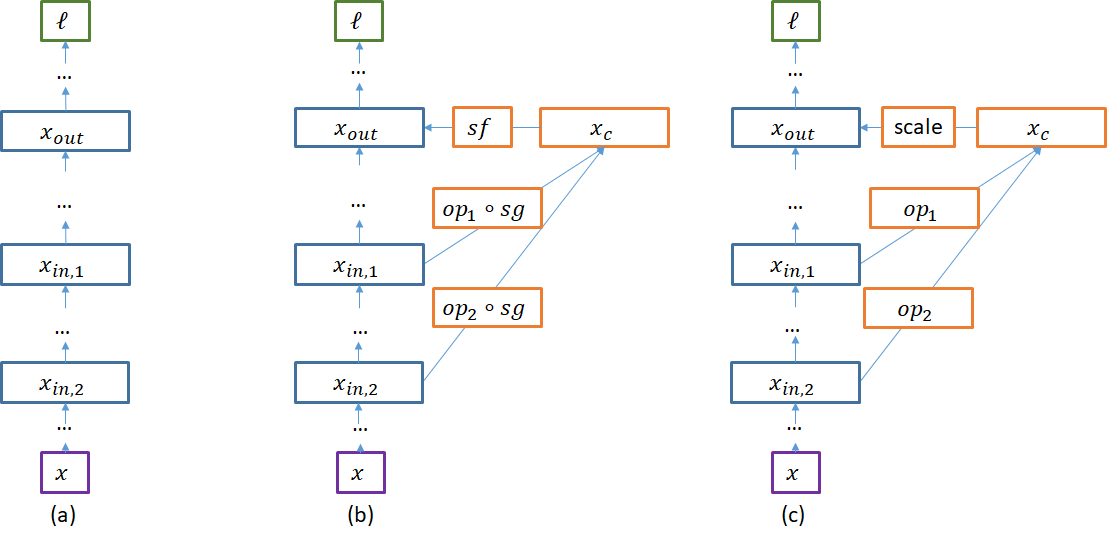
\includegraphics[keepaspectratio, width=0.8\textwidth]{img/hallu_steps.png}
    \caption{(a) Parent model.
    (b) Layer operations during candidate layer initialization step. $sg(x)$ is $x$ during forward and is zero during backward; $sf(x) = x - sg(x)$ is zero during forward, and computes gradient of $x$ during backpropagation; when a layer has multiple inputs, such as $x_c$, the inputs are summed together unless specified otherwise.
    (c) Layer operations of a finalized a candidate layer in a child model. 
    $scale(x)$ multiplies its input $x$ by a scalar, and the scalar is initialized as zero. }
    \label{fig:hallu_steps}
\end{figure*}


\subsection{Choice of Candidate Layers}
\label{sec:hallu_choice}

Since the number of possible candidate layers is large \todo{(how large)}, and we further allow multiple candidate layers to be added together to the parent model, the number of possible immediate children models of a fixed parent is astronomical. 
Hence if we use pure random sampling, the probability to find children in the top percentile is low \todo{(How low?)}. 

Instead, we propose in Fig.~\ref{fig:hallu_choice} to utilize feature selection and parameter sharing to initialize a combinatorial number of candidate layers and select a subset of them to form the candidate layer $x_c$ at the same time. For a given set of $x_{in,i}$, 



during the initialization phase to try a combinatorial number of candidate together and choose the most promising candidates.
 describes the high-level approach, and it is used as a generalization of Fig.~\ref{fig:hallu_steps}b. For each input $x_{in,i}$, we instantiate all possible operations to $x_{in,i}$, as $op_{i,1}, ..., op_{i,k}$, where $k$ is the maximum number of possible operations, which is typically around 5. Since we have $J$ input $x_{in,i}$, we a total of $Jk$ tensors $o_1, o_2, ..., o_{Jk}$. We simultaneously train these operations and learn to select a subset of them to be summed together to finalize the candidate layer $x_c$.

\begin{figure}[t]
    \centering
    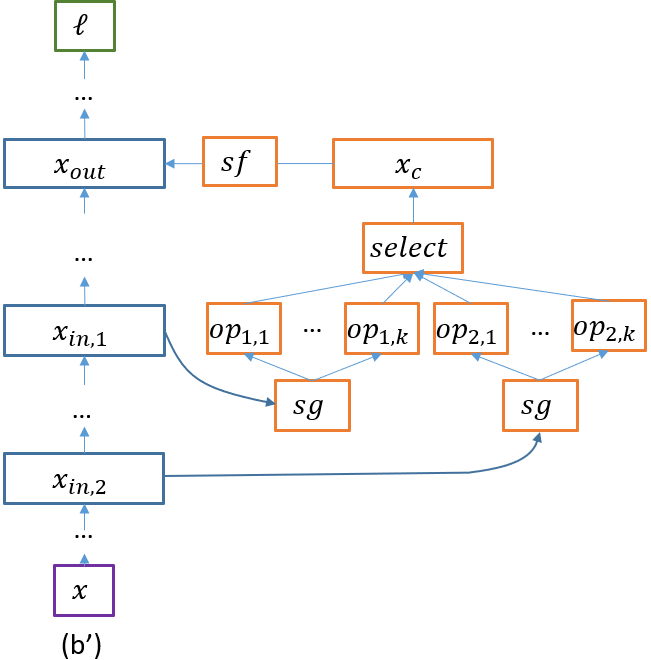
\includegraphics[width=0.8\linewidth, keepaspectratio]{img/hallu_choice.png}
    \caption{Initialize multiple operations together }
    \label{fig:hallu_choice}
\end{figure}

There are three important design choices to implement the proposed simultaneous feature selection and operation learning. 

\textbf{Candidate-parent Interaction.} 
The first choice is about whether we should allow candidate layers to affect the parent model while it is learning and initializing. 
Freezing the parent or using $sf$-$sg$ as pre- and post-fix of the candidate layer can allow us make the interaction non-existent, making the candidate layers converge faster potentially. However, it also reduces the expressive power of the candidates, and we have to formulate additional objectives for the candidates during initialization (we  show that that $sf$-$sg$ is in fact solving an optimization problem in Eq.~\ref{eq:linear_lasso}). We denote this option \textit{hard} since it hard stops the interaction between candidates and parents.

On the other hand, allowing the value freely flow between parent and candidate layers allow the new candidates to directly contribute to fitting the final loss. However, their initial value could be too far away from optimal in comparison to models in the parent, and it could negatively affect the parent models. Such problem is often encountered in literature that uses fine-tuning and more recently, learning without forgetting~\citep{}. The conventional wisdom of fine-tuning is to initialize the new (candidate) layers using learning rate that is much smaller than that used in training the parent model (0.1$\sim$0.02 times the original). We call this option \textit{soft} as it allows the interaction, but keep it at a slower rate. 

\textbf{Choice of Input Layers.} 
Choosing the inputs is a challenging problem since at depth $i$, there are $i-1$ potential earlier layers and any subset can be chosen. Any learning algorithm will have trouble explore and exploit the exponential number of choices without further assumptions. Hence, the most successful architecture search so far all opt to limit the input options by learning only a repeatable cell module and deploy the cell to a manually designed skeleton macro structure. Layers in a cell modules can only take input from other layers in the same cell and from the outputs of the two most recent previous cells. We also apply this option, and call it \textit{recent}. 
Recent works on skip connection patterns~\citep{logdense, sparsenet} have shown that sparse but well-placed skip connections can improve network accuracy. We call this option \textit{sparse}, and study them in experiments. \todo{implement log-dense}

\textbf{Choice of Operations on Inputs.}

As in Fig.~\ref{fig:hallu_choice}, we formulate the choice of operations as a feature selection problem. For each of the $J$ input layers, each generate $k$ operations, to form
operation tensor $o_1,...,o_{Jk}$, and the candidate $x_c$ is to sum a few of them with $x_c = select(o_1,..., o_{Jk}) = \sum _{j = 1}^{Jk} \omega_j o_j$. 

We consider three approaches for this feature selection problem.

\subsubsection{Lasso} 
One approach to achieve sparse feature selection is to linear combine the choices $o_1,...,o_{Jk}$ and use $L$-1 norm regularization on the linear weights. This is commonly known as Lasso
~\citep{lasso}. In our setting, we enforce the sparsity by adding the following regularization to the overall loss,
\begin{align}
    \lambda_{out} \sum _{j = 1}^{Jk} | \omega_j |,
\end{align}
where $\lambda_{out}$ is a parameter associated with $x_{out}$ to manage the level of sparsity. 

Since the stop-forward and stop-gradient operations stop the influence between the parent model and the candidate operations, we note that the candidate initialization and sparse selection is in fact solving the following $L$-1 regularized linear loss. 
\begin{align}
\label{eq:linear_lasso}
\min _{
    \substack{o_1,...,o_{Jk}, \\ \omega_1,..., \omega_{Jk}}
    } 
    E [\langle 
        \frac{\partial \ell}{\partial x_{out}} , 
        \sum _{j = 1}^{Jk} \omega_j o_j
    \rangle ] 
    + \lambda_{out} \sum _{j = 1}^{Jk} | \omega_j |,
\end{align}
where the expectation is taken over the distribution of input samples. 
To see that our candidate initialization solves the above optimization, we note that the gradient of the first term with respect to $o_j$ is the gradient that we will update $o_j$ with in Fig.~\ref{fig:hallu_choice} due to the $sf$ operation after $x_c$. 

\subsubsection{$L$-2 fitting of the gradient}
Eq.~\ref{eq:linear_lasso} matches the candidate output $x_c$ to the target negative gradient $-\frac{\partial \ell}{\partial x_{out}}$ minimizing a linear loss. Here we consider replacing the linear loss with square loss as follows.
\begin{align}
\min _{
    \substack{o_1,...,o_{Jk}, \\ \omega_1,..., \omega_{Jk}}
    } 
    \frac{1}{2}E \big[ 
     \Vert 
        - \frac{\partial \ell}{\partial x_{out}} - 
        \sum _{j = 1}^{Jk} \omega_j o_j
    \Vert^2_2 \big] 
    + \lambda_{out} \sum _{j = 1}^{Jk} | \omega_j |, 
\end{align}
which is equivalent to 
\begin{align}
\label{eq:quadratic_lasso}
\min _{
    \substack{o_1,...,o_{Jk}, \\ \omega_1,..., \omega_{Jk}}
    } 
    E [\langle 
        \frac{\partial \ell}{\partial x_{out}} , 
        x_c
    \rangle 
    + \frac{1}{2} \Vert x_c \Vert^2_2] 
    + \lambda_{out} \sum _{j = 1}^{Jk} | \omega_j |.
\end{align}
\todo{The L-2 regularization seem to incur problems on the parent model. (should not happen). This may be because the global norm of gradient is clipped; there are some hidden connections that makes the $sf$-$sg$ ineffective.  }


\textbf{Direct Training with Backpropagation.}





    
\section{Experiment}

%%%%%%%%%%%%%%%%%%%%%%%% 
% Experimental questions
%%%%%%%%%%%%%%%%%%%%%%%%
\subsection{Experimental questions}
\begin{enumerate}
\item Parent model choices ablation study (Sec.~\ref{sec:greedy_vs_convex})
\item Hallucination initialization ablation study. (Sec.~\ref{sec:soft_vs_hard})
\item Cell based search versus macro search (Sec.~\ref{sec:cell_vs_macro})
\item How many subsets should we try out given each hallucination batch? (Few is good see Sec.~\ref{sec:n_select_per_init}.)
\item What's the ratio between initialized hallucinated operations and the number selected in the selected subset?
    
\end{enumerate}


%%%%%%%%%%%%%%%%%%%%%%%% 
% Data-sets
%%%%%%%%%%%%%%%%%%%%%%%%
\subsection{Experiment Set-up and Data-sets}

\begin{enumerate}
    \item CIFAR10, CIFAR100
    \item OpenML 500
\end{enumerate}


%%%%%%%%%%%%%%%%%%%%%%%% 
% Eval metric
%%%%%%%%%%%%%%%%%%%%%%%%
\subsection{Evaluation Metrics}

\begin{enumerate}
    \item For fixed search space and training parameters, we can 
    compare the best found model validation error after the same number of 
    models are trained.
    \item For a more general comparison among search algorithms, we plot the curves of the best validation error versus FLOPs spent on training. Then the lower curves represent algorithms that find the most accurate models faster.
    \item While the previous two metrics focus on how fast the search can find the most accurate models, they do not consider the cost-efficiency of the searched models. To evaluate the cost-efficiency, we represent the cost-efficiency of searched models by the lower convex hull of validation error versus model computational cost, measured in FLOPs. The more close the hull is to the origin, the more cost efficient the found models are. We can compare algorithms by comparing their performance convex hulls. 
\end{enumerate}


%%%%%%%%%%%%%%%%%%%%%%%% 
% Parent choice Experiment
%%%%%%%%%%%%%%%%%%%%%%%%
\subsection{Greedy versus Convex Hull}
\label{sec:greedy_vs_convex}

In Sec.~\ref{sec:parent_choice} we propose a method, Convex, to expand parent models that are near the lower performance convex hull of all trained models. This section compares this method against a naive greedy strategy (Greedy), where models that are close to be the most accurate models are selected to be the parent models. Fig.~\ref{fig:convex_hull_vs_greedy} compares the two methods by how fast they can find accurate models, and we observe that Convex can achieve more accurate models faster than Greedy. We also compare the final performance convex hulls of the two methods in Fig.~\ref{fig:perf_ch}, and we notice that Greedy suffers when models are larger. This is possibly because the greedy exploration does not have the ability to backtrack to earlier models, and may stuck at local optimum.

\begin{figure}[t]
    \centering
    \subfloat[CIFAR10]{
       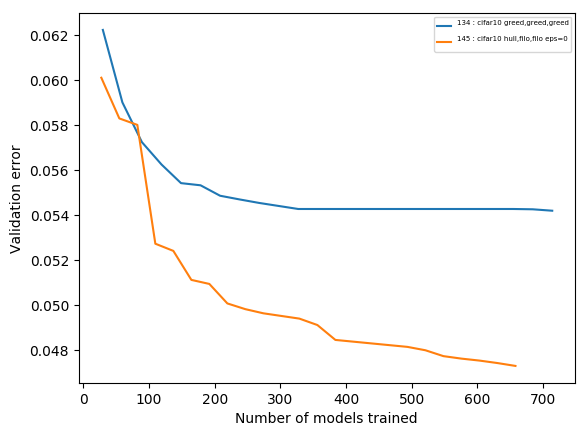
\includegraphics[width=0.8\linewidth, keepaspectratio ]{img/cust_exps_134_145.png}
        \label{fig:convex_hull_vs_greedy_cifar10}
    }
    
    \subfloat[CIFAR100]{
       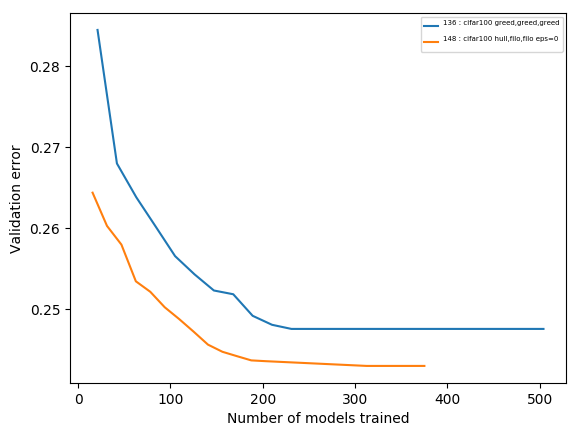
\includegraphics[width=0.8\linewidth, keepaspectratio ]{img/cust_exps_136_148.png}
        \label{fig:convex_hull_vs_greedy_cifar100}
    }
    
    \caption{Orange expands models that are on the performance convex hull, 
    blue expands models that are the most accurate so far. By focusing on the cost-efficiency instead of the accuracy alone, we found that expanding at the performance convex hull results in more accurate models with the 
    same number of trials. }
    \label{fig:convex_hull_vs_greedy}
\end{figure}

\begin{figure}[t]
    \centering
    \subfloat[CIFAR10]{
    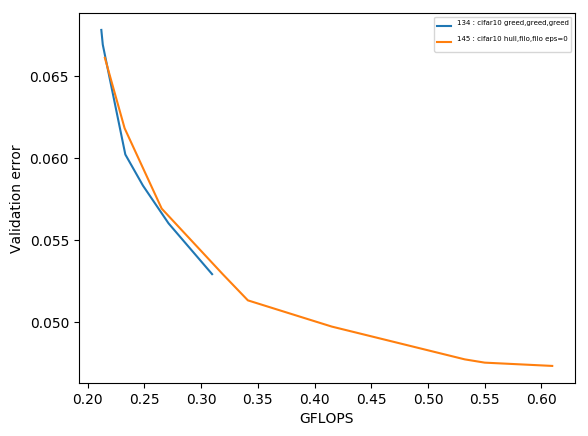
\includegraphics[width=0.8\linewidth, keepaspectratio ]{img/cust_exps_134_145_final_CH.png}
    \label{fig:perf_ch_cifar10}
    }
    
    \subfloat[CIFAR100]{
    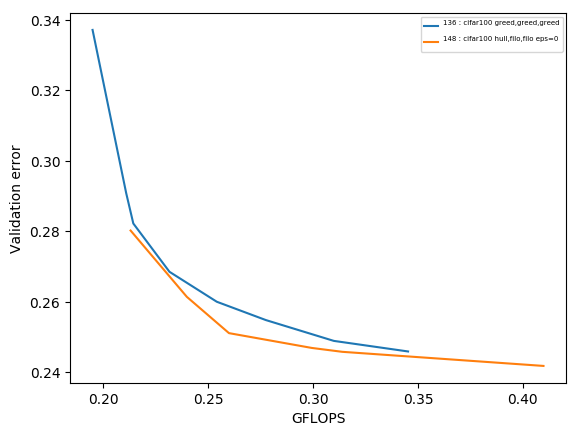
\includegraphics[width=0.8\linewidth, keepaspectratio ]{img/cust_exps_136_148_final_CH.png}
    \label{fig:perf_ch_cifar100}
    }
    \caption{The performance convex hull of Greedy (blue) and Convex(orange). 
    We observe that Greedy seem to be more easily stuck at local minimum, 
    so that its final models are not as accurate as those of Convex.}
    \label{fig:perf_ch}
\end{figure}

%%%%%%%%%%%%%%%%%%%%%%%% 
% Hallu init Experiment
%%%%%%%%%%%%%%%%%%%%%%%%
\subsection{Candidate Initialization Ablation Study}
\label{sec:soft_vs_hard}

In Sec.~\ref{sec:hallu_init} we propose to initialize candidate layer parameters in a initialization phase, in which the candidate layers cannot affect the parent model in neither forward or backward operations. We call this approach \emph{hard} initialization, since it strictly prevents any influence of the candidate on the parental models. This section compares hard initialization against \emph{soft} initialization, where we add the candidate layer to the parent model directly using Fig.~\ref{fig:hallu_steps}c. We note that soft initialization is a naive net-morphism~\citep{netmorph}, where the candidate layers are randomly initialized, and its scale is initially zero, so it initially does not affect the parent model. 
Fig.~\ref{fig:soft_vs_hard} compares the two initialization method for search, and we observe that hard initialization is faster than soft to find more accurate models.

\todo{To compare initialization quality, we should form several fixed sequence of models, and compare the accuracy of training them incrementally using soft and hard initializations.}


\begin{figure*}[t]
    \centering
    \subfloat[cell cifar10]{
        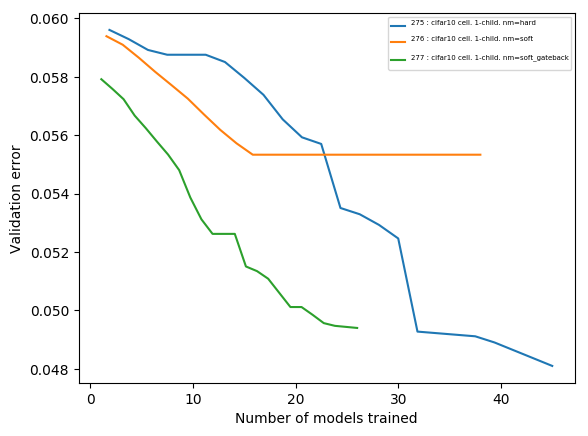
\includegraphics[width=0.4\linewidth, keepaspectratio ]{img/cust_exps_275_276_277.png}
        \label{fig:soft_vs_hard_cifar10}
    }
    ~
    \subfloat[cell cifar100]{
        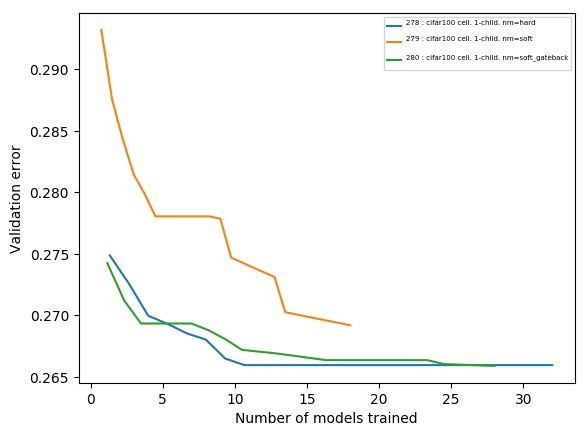
\includegraphics[width=0.4\linewidth, keepaspectratio ]{img/cust_exps_278_279_280.png}
        \label{fig:soft_vs_hard_cifar100}
    }
    
    \subfloat[macro cifar10 starting from NasNet-A]{
        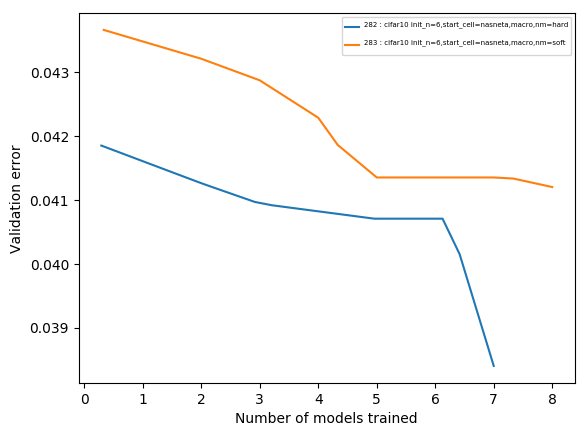
\includegraphics[width=0.4\linewidth, keepaspectratio ]{img/cust_exps_282_283.png}
        \label{fig:soft_vs_hard_cifar10_macro}
    }
    ~
    \subfloat[macro cifar100 starting from NasNet-A]{
        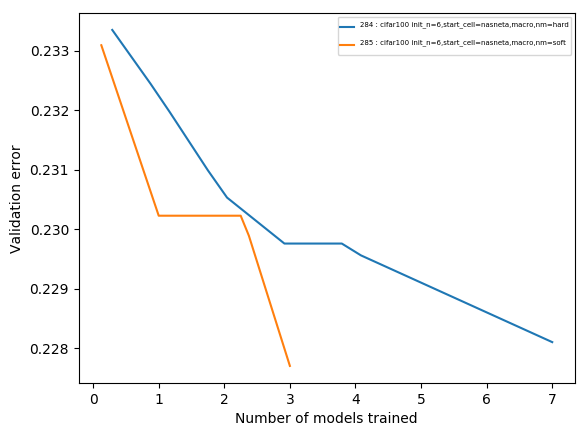
\includegraphics[width=0.4\linewidth, keepaspectratio ]{img/cust_exps_284_285.png}
        \label{fig:soft_vs_hard_cifar100_macro}
    }
    
    \caption{Caption}
    \label{fig:soft_vs_hard}
\end{figure*}


%%%%%%%%%%%%%%%%%%%%%%%% 
% Cell vs Macro Experiment
%%%%%%%%%%%%%%%%%%%%%%%%
\subsection{Incremental Training Ablation Study}
\label{sec:incremental_vs_from_scratch}
In Sec.~\ref{sec:hallu_init} we propose to train children models starting from existing parent model parameters. While the early architecture search literature~\citep{} trains each new model from scratch for few epochs to evaluate them, it has been argued that such approach is inaccurate in evaluating the models~\citep{}. In fact, the more recent literature~\citep{} favors reusing parent model parameters over training from scratch, and leads to faster searches. 
This section showcases that when exploring the search tree of models, we should use incremental training over training from scratch, because the former can approximate the true accuracy of the models much closer, while using significantly fewer training time per model. Furthermore, incremental training can reduce the extra training phase to the final models, a phase that is required for methods that train models from scratch for only few epochs.  

To compare the two child model training methods, We randomly sample a sequence of candidate layers, and add them to the model one at a time. We train two copies for each model. One is from scratch for 300 epochs. The other inherits its parent's parameters, and it is trained for 40 epochs, while initializing the next candidate layer at the same time. The initial model is randomly initialized. Fig.~\ref{fig:inc_vs_scratch} shows sequence indices versus error rates that are averaged over 10 sequences. We observe that incremental training is able to quickly overcome the initial disadvantage of having few training epochs, and is able to achieve lower error rates later in the sequences. This also suggests that complex models  during search are difficult to train well from scratch, but incremental training allows us to train them using fewer epochs while getting better accuracy. Furthermore, since the number of possible models grow exponentially with the search tree depths, the majority of models are more accurately and more quickly trained using incremental than from-scratch training.

\todo{Same comparison but start with trained model?}

\begin{figure}[t]
    \centering
    \subfloat[CIFAR10 Incremental vs. From-scratch]{
    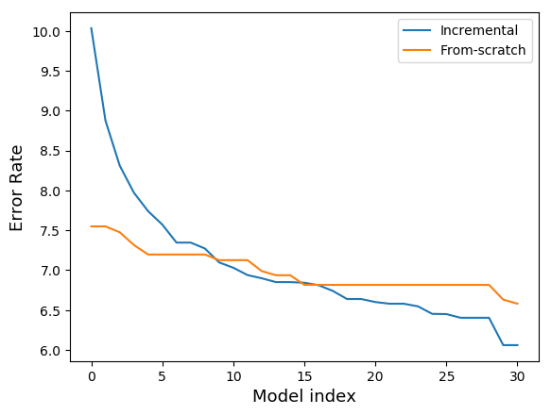
\includegraphics[keepaspectratio,width=0.8\linewidth]{img/inc_vs_scratch_cifar10.png}
    \label{fig:inc_vs_scratch_cifar10}
    }
    
    \subfloat[CIFAR100 Incremental vs. From-scratch]{
    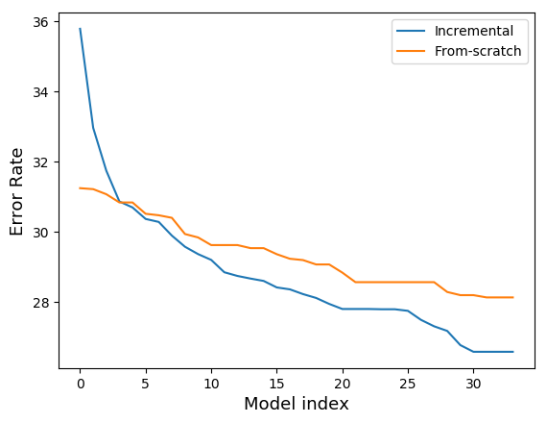
\includegraphics[keepaspectratio,width=0.8\linewidth]{img/inc_vs_scratch_cifar100.png}
    \label{fig:inc_vs_scratch_cifar100}
    }
    \caption{Incremental training versus from-scratch training.}
    \label{fig:inc_vs_scratch}
\end{figure}


%%%%%%%%%%%%%%%%%%%%%%%% 
% Cell vs Macro
%%%%%%%%%%%%%%%%%%%%%%%%
\subsection{Cell Versus Macro search}
\label{sec:cell_vs_macro}

The current results show that cell based search to be much faster to reach the same 
accuracy level than macro structure search in Fig.~\ref{fig:cell_vs_macro_cifar10}.
Furthermore, the final performance convex hull of the cell based search also displays better cost efficiency than those of the macro structure searches in Fig.~\ref{fig:cell_vs_macro_cifar10_final_CH}. 

\todo{One possible reason that still need to be rule out is that macro searches takes smaller steps due to the number of hallucination selected. Furthermore, the known macro search starts with models that are worse than the starting points of cell based searches. Do macro searches that have the same branching and same starts as 275..280}


\begin{figure}[t]
    \centering
    \subfloat[Cell vs. Macro]{
        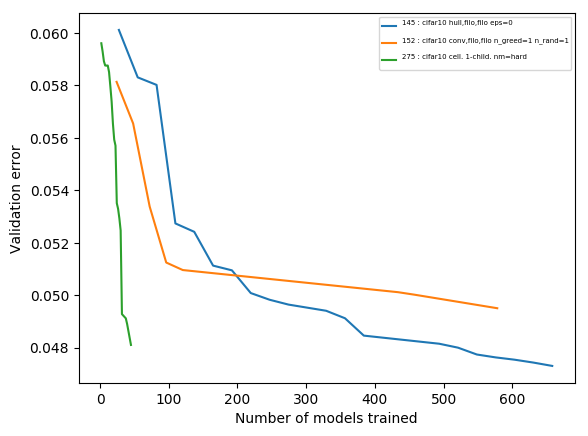
\includegraphics[width=0.8\linewidth, keepaspectratio ]{img/cust_exps_145_152_275.png}
        \label{fig:cell_vs_macro_cifar10}
    }
    
    \subfloat[Cell vs. Macro Performance Convex Hull]{
        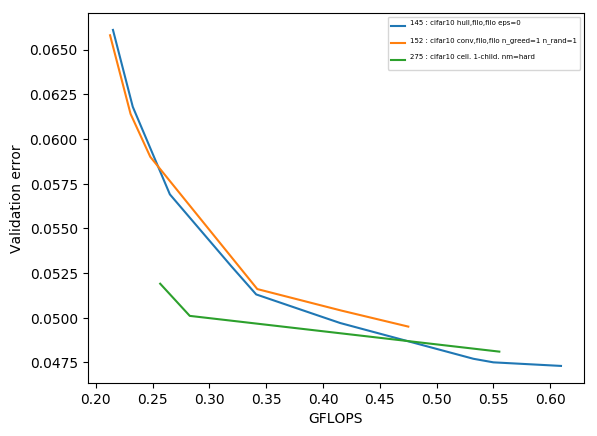
\includegraphics[width=0.8\linewidth, keepaspectratio ]{img/cust_exps_145_152_275_final_CH.png}
        \label{fig:cell_vs_macro_cifar10_final_CH}
    }
    \caption{Caption}
    \label{fig:cell_vs_macro}
\end{figure}



%%%%%%%%%%%%%%%%%%%%%%%% 
% Search tree parameter
%%%%%%%%%%%%%%%%%%%%%%%%
\subsection{Number of children after each batch of hallucination initialization}
\label{sec:n_select_per_init}



\begin{figure*}[t]
    \centering
    
    \subfloat[cifar10]{
        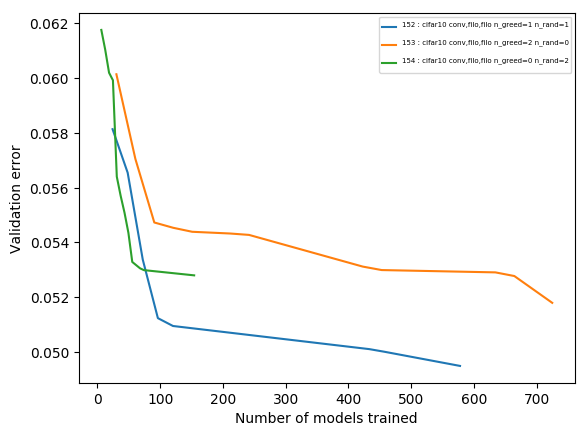
\includegraphics[width=0.4\linewidth, keepaspectratio ]{img/cust_exps_152_153_154.png}
        \label{fig:num_greedy_vs_num_rand_cifar10}
    }
    ~
    \subfloat[cifar100]{
        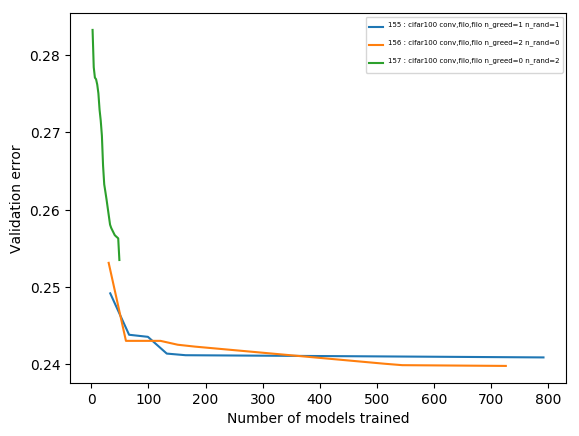
\includegraphics[width=0.4\linewidth, keepaspectratio ]{img/cust_exps_155_156_157.png}
        \label{fig:num_greedy_vs_num_rand_cifar100}
    }
    
    \subfloat[cifar10]{
        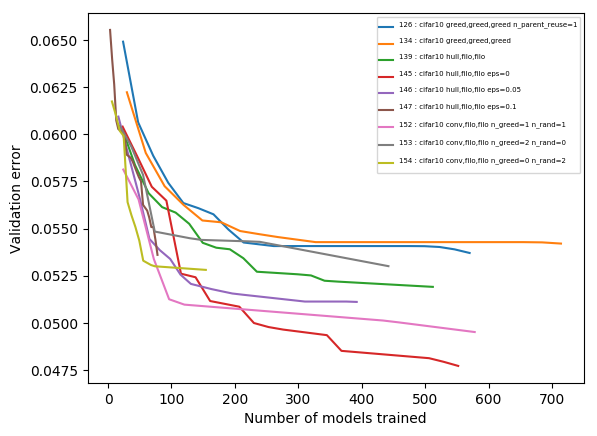
\includegraphics[width=0.4\linewidth, keepaspectratio ]{img/cust_exps_145_146_147_139_126_134_152_153_154.png}
        \label{fig:num_branch_cifar10}
    }
    ~
    \subfloat[cifar100]{
        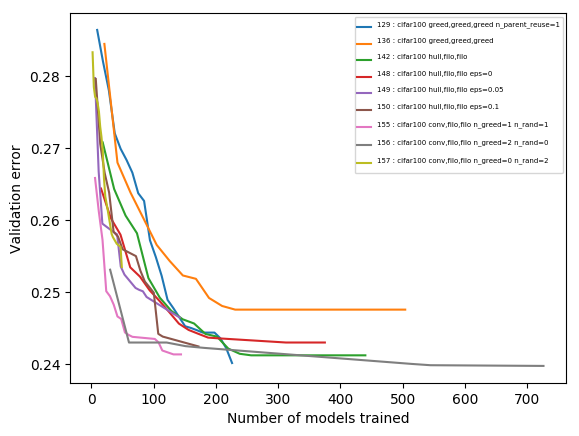
\includegraphics[width=0.4\linewidth, keepaspectratio ]{img/cust_exps_148_149_150_142_129_136_155_156_157.png}
        \label{fig:num_branch_cifar100}
    }
    \caption{}
    \label{fig:num_branch}
\end{figure*}



\section{TODOs}
\begin{enumerate}
    \item random chances of being good /bad due to warm starts
    \item avoid sampling the same hallus?
    \item training flops (petridish/analysis/search\textunderscore analysis)
    \item Pareto vs Convex?
    \item Update hallu handling for macro. 
\end{enumerate}



%\nocite{langley00}

\bibliographystyle{sty_bst/icml.bst}
\bibliography{network_search}

\appendix
\section{Model details}
\label{sec:petridish_layer_info}

\end{document}
